\setcounter{chapter}{-1}
\renewcommand{\thechapter}{\Roman{chapter}}
\counterwithout{section}{chapter} 
\counterwithout{subsection}{chapter}

\chapter{Introduction}



\section{Le Portail Pro.one.be}
Le portail PRO.ONE a été conçu pour rassembler en un seul endroit toutes les informations nécessaires au suivi de vos dossiers d’agrément et de subvention gérés au niveau du département accueil de l’ONE. Vous y trouverez les portes d’entrée vers tous les secteurs dont vous dépendez. Derrière ce portail, une base de données unique contient l’ensemble des informations collectées. Cela signifie que vous encoderez désormais une seule fois les données même si elles sont utilisées à plusieurs niveaux.

Votre Portail est constitué du volet de navigation à gauche et de quelques raccourcis au centre (figure \ref{fig:home_page}).

\begin{figure}[h]
    \centering
    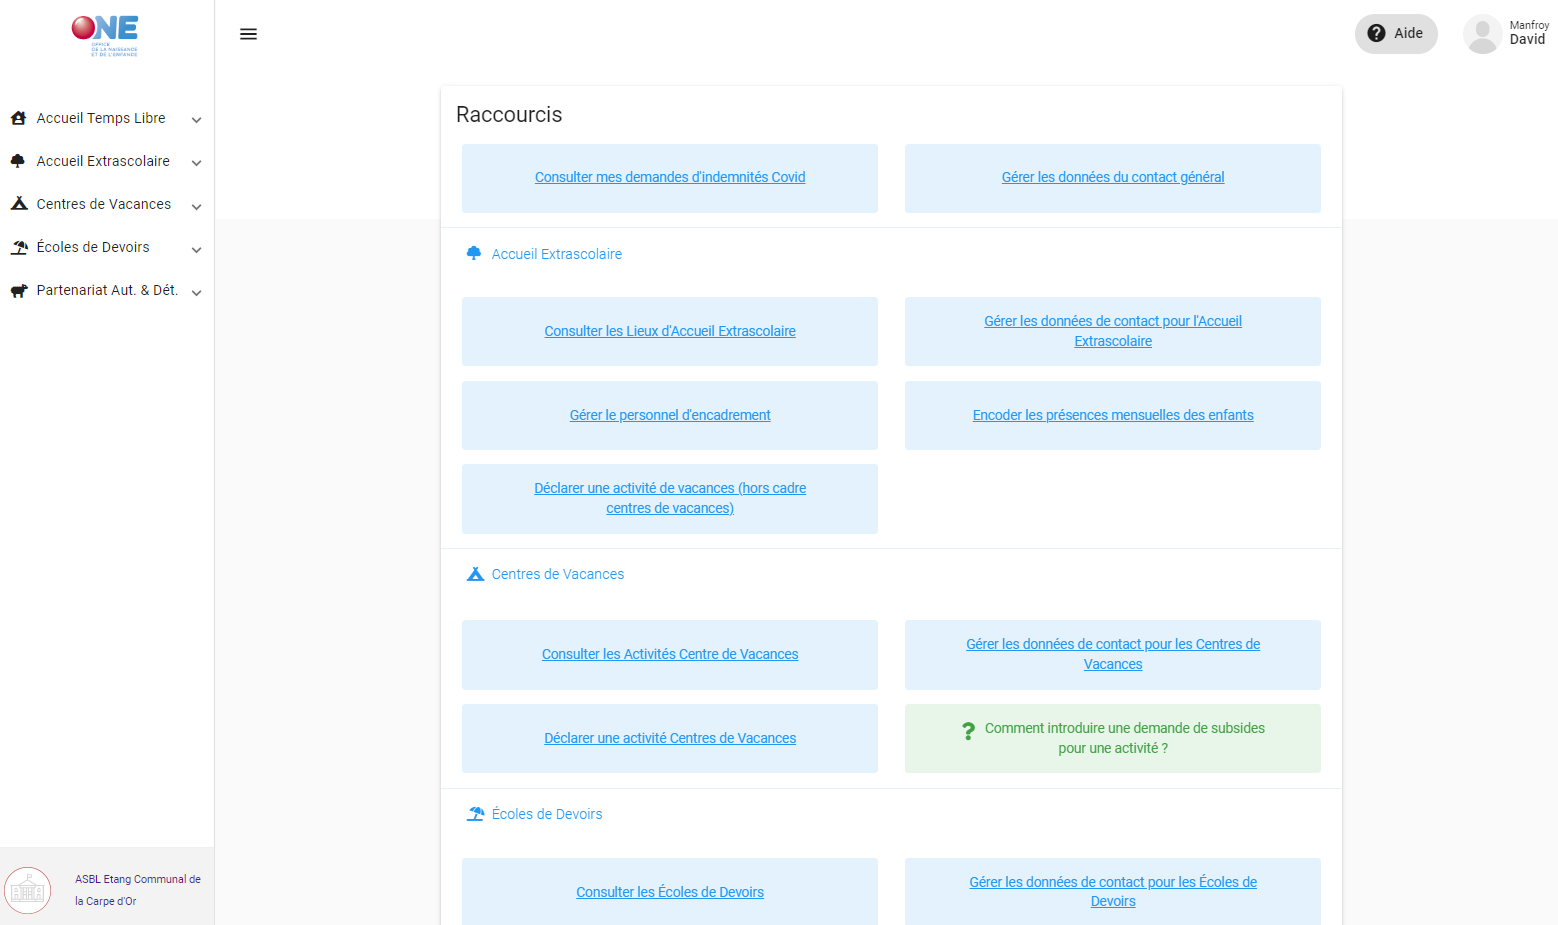
\includegraphics[width=16cm]{Images/intro/home_page.png}
    \caption{L'écran d'accueil présente un volet de navigation sur la gauche et des raccourcis au centre de l'écran.}
    \label{fig:home_page}
\end{figure}


\subsection{Le volet de navigation}
Pour cacher ou afficher le volet, cliquez sur les trois petites barres 
\includegraphics{Images/intro/button_volet.png}. Chaque entrée du volet peut se déplier. \textbf{Accueil Temps Libre}, vous donnera accès à des fonctionnalités transversales: \begin{itemize}
    \item \textbf{Indemnité COVID}: pour accéder au formulaire de demande d'indemnité COVID;
    \item \textbf{Contact général}: pour mettre à jour la personne de contact de votre pouvoir organisateur. Notez que vous pouvez spécifier une personne de contact différente pour chaque secteur. 
    \item \textbf{Mon Équipe}: où vous retrouverez l'ensemble de votre personnel d'encadrement. 
    \item \textbf{Utilisateur}: où vous retrouverez l'ensemble des personnes autorisées à se connecter au Portail Pro grâce à eID et/ou itsme.
\end{itemize}
Les autres entrées sectorielles possèdent chacune leur propres fonctionnalités.

\subsection{Les raccourcis}
Les boutons de raccourcis permettent d’accéder directement aux fonctionnalités le plus souvent utilisées.  

\section{Le Service support de l'ONE (pro@one.be)}
Le bouton aide en haut à droite de l'écran vous indique les coordonnées de contact de notre Service support (de première ligne). 

\begin{remarque} \label{helpdesk}
Ce service n'est pas compétent pour répondre aux questions qui concernent les procédures administratives de l'Accueil Temps Libre, mais pourra vous renseigner les coordonnées des personnes ressources (votre gestionnaire de dossiers par exemple). Le mieux pour les questions d’ordre administratif est d’appeler directement votre gestionnaire, votre conseillère ou le secrétariat de nos services.
\end{remarque}

\section{Accéder au Portail Professionnel}
Le Portail Professionnel est accessible à cette adresse: \url{https://pro.one.be} (\textit{à ne pas confondre avec le site institutionnel destiné au public} \url{https://www.one.be})\\
\centerline{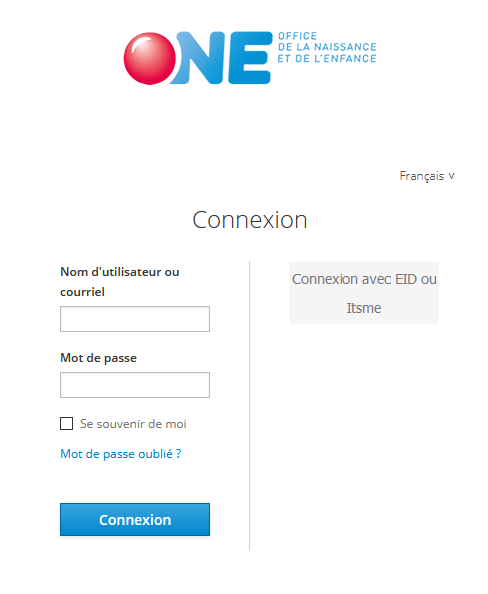
\includegraphics[width=5cm]{Images/intro/connexionPortail.png}}


\subsection{Navigateurs recommandés}
Pour des questions de compatibilité, nous recommandons d'utiliser les navigateurs à jour suivants:
\begin{itemize}
    \item Google Chrome (télécharger: \url{https://www.google.com/intl/fr/chrome/})
    \item Mozilla Firefox (télécharger: \url{https://www.mozilla.org/fr/firefox/new/})
\end{itemize}


\section{Se connecter au Portail Pro via It's me ou eID}
\begin{information}
Pour avoir accès au Portail Pro.one.be via It's me ou eID, contactez l'administrateur de votre pouvoir organisateur.
\end{information}
Cliquez sur Connexion avec eID ou It's me. Le Portail Pro vous renvoie vers le Portail CSAM - S'identifier à l'administration en ligne pour que vous puissiez vous identifier. Cliquez ensuite sur le moyen de connexion que vous souhaitez utiliser (carte d'identité ou application It's me) (voir fig. \ref{fig:CSAM_portal}). 


\begin{figure}
    \centering
    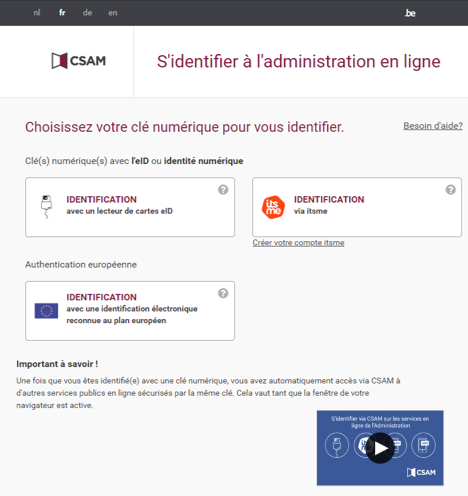
\includegraphics[width=8cm]{Images/intro/csam.png}
    \caption{Portail CSAM permettant de se connecter au Portail Pro.one.be}
    \label{fig:CSAM_portal}
\end{figure}


\subsection*{Se connecter au Portail via l'identifiant par défaut: nom d'utilisateur, mot de passe}

\begin{attention}
L'identifiant par défaut sera bientôt \textcolor{rouge}{désactivé} au profit d'une connexion forte via eID ou It's me. Demandez à l'administrateur de votre organisation de configurer vos accès eID ou It's me.  
\end{attention}

Si votre administrateur n'a pas encore configuré votre accès eID ou It's me, vous pouvez utiliser la connexion via \textbf{l'identifiant par défaut}. L'identifiant par défaut est unique pour l'organisation. Il vous donne accès à l'accueil de la Petite Enfance (crèche, accueillantes, maison d'enfants, etc.) et l'accueil Temps Libre (centres de vacances, écoles de devoirs, accueil extrascolaire).

\subsubsection{Oubli de votre identifiant par défaut}
Si vous avez oublié votre identifiant par défaut (nom d'utilisateur - mot de passe), vous pouvez contacter notre Service Support à l'adresse pro@one.be. Précisez bien votre Pouvoir organisateur, et si besoin, le numéro d'entreprise (BCE) afin que l'on puisse mieux vous retrouver dans notre base de données. Notre Service support vous octroiera un nouveau mot de passe temporaire. Vous serez invité à le changer lors de votre connexion. Nous vous demandons également de communiquer l'identifiant et le nouveau mot de passe à tous les services susceptibles de se connecter au Portail \url{https://Pro.one.be}. 

\subsubsection{Mettre à jour les informations de votre identifiant par défaut}
Vous pouvez mettre à jour l'affichage du nom et du prénom associé à l'identifiant en vous rendant sur \url{https://login.one.be}. Vous pourrez également mettre à jour le mail de connexion et changer votre mot de passe.



\counterwithin{section}{chapter}
\counterwithin{subsection}{chapter}
\renewcommand{\thechapter}{\arabic{chapter}}









